%source: Path: /mnt/9636D17436D15639/University/Ta/Logic/Design/Utils/Adel/Ehb205e-2021-fall-quiz-02.pdf




مدار شکل زیر را درنظر بگیرید، این مدار یه ورودی \lr{A} و \lr{B} و \lr{CLK} و دو خروجی \lr{X} و \lr{Y} دارد. جدول مشخصه\footnote{\lr{Characteristic Table}} و جدول درستی\footnote{\lr{Truth Table}} و معادلات بولی خروجی‌های \lr{X} و \lr{Y} را بنویسید.



\begin{figure}[h]
	\centering
	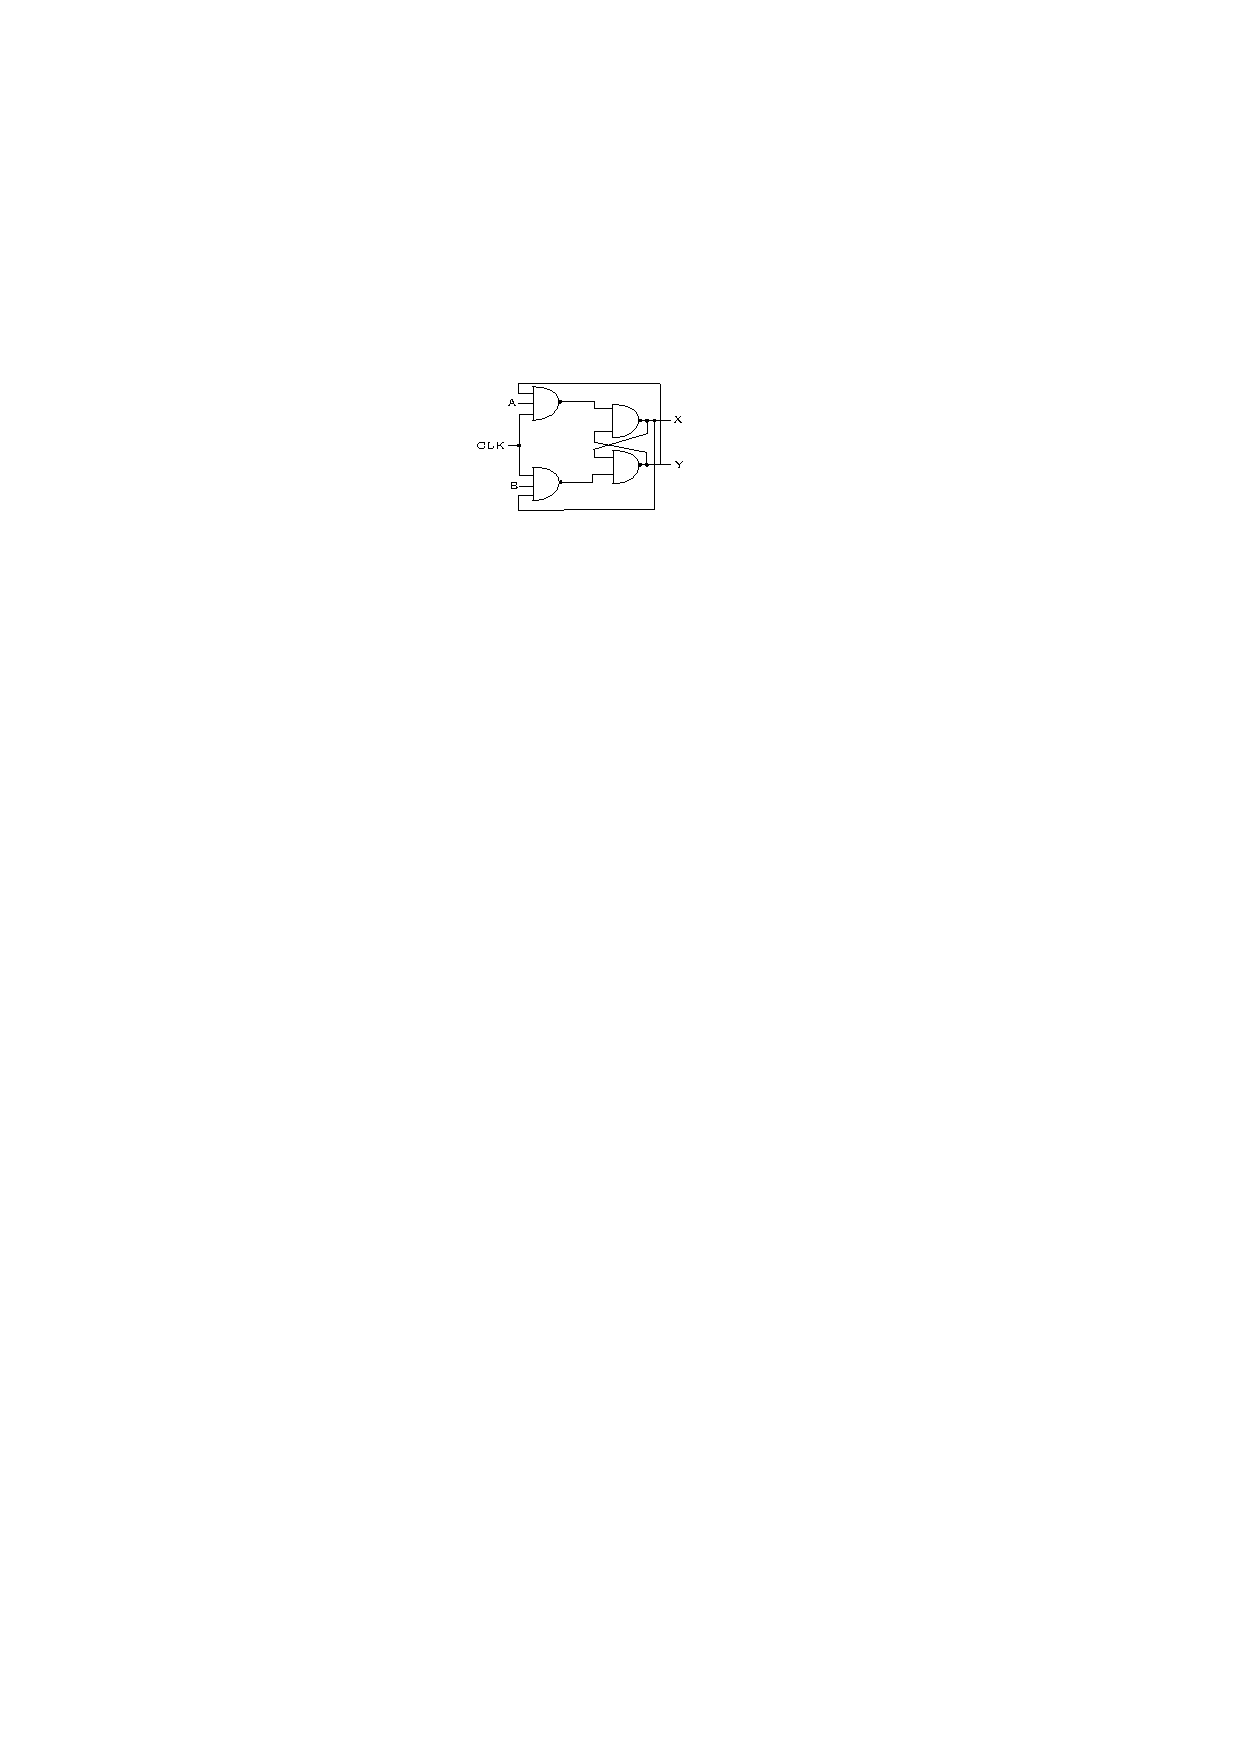
\includegraphics[width=0.4\textwidth]{fig/Q_opt1.pdf}
	\label{fig:Q_opt_1}
\end{figure}












%source: AUT-CE-LC HW10-Q1
%مدار شکل زیر را تحلیل کرده و جدول مشخصه\footnote{\lr{Characteristic Table}} آن را رسم کنید.
%
%
%
%\begin{figure}[h]
%	\centering
%	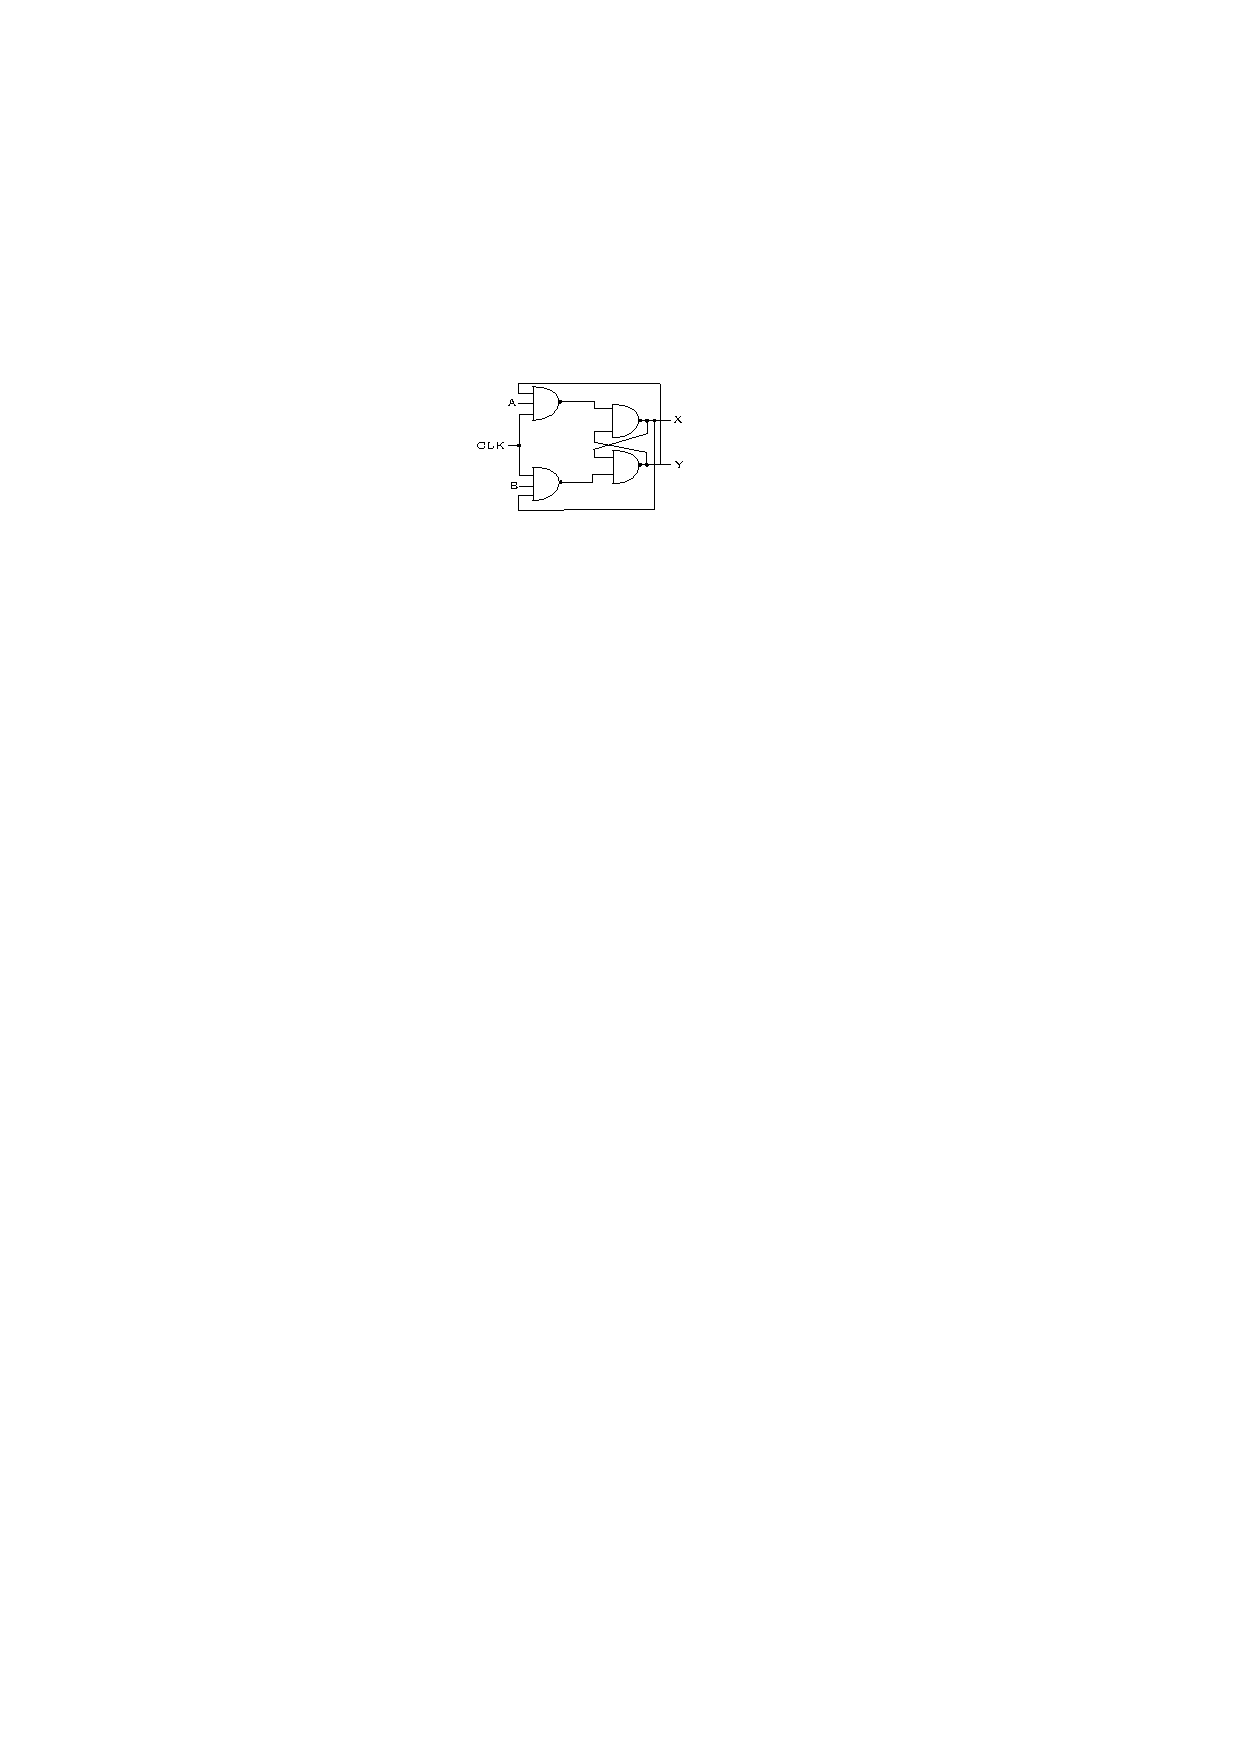
\includegraphics[width=0.4\textwidth]{fig/Q_opt1.pdf}
%	\label{fig:Q_opt_1}
%\end{figure}
